\documentclass[submit]{harvardml}

% Put in your full name and email address.
\name{Luke Mueller}
\email{lam908@mail.harvard.edu}

% List any people you worked with.
\collaborators{%
  Dong Yan
}

% You don't need to change these.
\course{CS181-S16}
\assignment{Assignment \#5}
\duedate{5:00pm April 15, 2016}

\usepackage[OT1]{fontenc}
\usepackage[colorlinks,citecolor=blue,urlcolor=blue]{hyperref}
\usepackage[pdftex]{graphicx}
\usepackage{subfig}
\usepackage{fullpage}
\usepackage{palatino}
\usepackage{mathpazo}
\usepackage{amsmath}
\usepackage{amssymb}
\usepackage{color}
\usepackage{todonotes}
\usepackage{listings}
\usepackage{common}
\usepackage{bm}
\usepackage{enumitem}

\usepackage[mmddyyyy,hhmmss]{datetime}

\definecolor{verbgray}{gray}{0.9}

\lstnewenvironment{csv}{%
  \lstset{backgroundcolor=\color{verbgray},
  frame=single,
  framerule=0pt,
  basicstyle=\ttfamily,
  columns=fullflexible}}{}

\begin{document}
\begin{center}
{\Large Homework 5: EM for a Simple Topic Model}\\
\end{center}

There is a mathematical component and a programming component to this homework.
Please submit ONLY your PDF to Canvas, and push all of your work to your Github
repository. If a question requires you to make any plots, please
include those in the writeup.

\begin{mdframed}[style=exampledefault]
\textbf{Background:} In this homework, you will implement a very simple kind of topic model.  Latent Dirichlet allocation, as we discussed in class, is a topic model in which each document is composed of multiple topics.  Here we will make a simplified version in which each document has just a single topic.  As in LDA, the vocabulary will have~$V$ words and a topic will be a distribution over this vocabulary.  Let's use~$K$ topics and the~$k$th topic is a vector~$\bbeta_k$, where~${\beta_{k,v}\geq 0}$ and~${\sum_v \beta_{k,v}=1}$.  Each document can be described by a set of word counts~$\boldw_{d}$, where~$w_{d,v}$ is a nonnegative integer.  Document~$d$ has~$N_d$ words in total, i.e.,~${\sum_v w_{d,v}=N_d}$.  Let's have the unknown overall mixing proportion of topics be~$\btheta$, where~${\theta_k\geq 0}$ and~${\sum_k\theta_k=1}$.  Our generative model is that each of the~$D$ documents has a single topic~${z_d\in \{1,\ldots,K\}}$, drawn from~$\btheta$; then, each of the words is drawn from~$\bbeta_{z_d}$.

\end{mdframed}

%%%%%%%%%%%%%%%%%%%%%%%%%%%%%%%%%%%%%%%%%%%%%
% Problem 1
%%%%%%%%%%%%%%%%%%%%%%%%%%%%%%%%%%%%%%%%%%%%%
\begin{problem}[Complete Data Log Likelihood, 4 pts]

Write the complete-data log likelihood~$\ln p(\{z_d,\boldw_d\}^D_{d=1}\given\btheta, \{\bbeta_k\}^K_{k=1})$. It may be convenient to write~$z_d$ as a one-hot coded vector~$\boldz_d$.


\end{problem}
\subsection*{Solution}
Using properties of the joint distribution, we can rewrite the complete-data log likelihood as:
\[
\ln p(\{z_d,\boldw_d\}^D_{d=1}\given\btheta, \{\bbeta_k\}^K_{k=1}) = \ln \big[ p(\{z_d\}^D_{d=1} \given \btheta) \times p(\{\boldw_d\}^D_{d=1} \given \{z_d\}^D_{d=1}, \{\bbeta_k\}^K_{k=1}) \big] \
\]

\noindent
Then dealing with the terms separately, we have:
\begin{align*}
\ln p(\{z_d\}^D_{d=1} \given \btheta) & = ln \prod_{d=1}^{D} \btheta = ln \prod_{d=1}^{D} \prod_{k=1}^{K} \theta_k \ \\
\ln p(\{\boldw_d\}^D_{d=1} \given \{z_d\}^D_{d=1}, \{\bbeta_k\}^K_{k=1}) & = \ln \prod_{d=1}^{D} \bbeta =  ln \prod_{d=1}^{D} \prod_{k=1}^{K} \beta_k 
= ln \prod_{d=1}^{D} \prod_{k=1}^{K} \prod_{v=1}^{V} \beta_{k,v}^{w_{d,v}}
\end{align*}

\noindent
Then combining terms again, and making use of $z_d$ as a one-hot coded vector~$\boldz_d$:

\begin{align*}
\ln p(\{z_d,\boldw_d\}^D_{d=1} \given\btheta, \{\bbeta_k\}^K_{k=1}) & = \prod_{d=1}^{D} \prod_{k=1}^{K} \theta_k^{z_{dk}} \prod_{v=1}^{V} (\beta_{kv})^{w_{dv}z_{dk}} \\
& = \sum_{d=1}^{D} \sum_{k=1}^{K} \big[ z_{dk} \ln (\theta_k) + \sum_{v=1}^{V} z_{dk} w_{dv} \ln (\beta_{kv}) \big] \\
& = \sum_{d=1}^{D} \sum_{k=1}^{K}  z_{dk} \big[\ln (\theta_k) + \sum_{v=1}^{V} w_{dv} \ln (\beta_{kv}) \big]
\end{align*}




\newpage
\begin{problem}[Expectation Step, 5pts]

Introduce estimates~$q(\boldz_d)$ for the posterior over the hidden variables~$\boldz_d$.  What did you choose and why?  Write down how you would determine the parameters of these estimates, given the observed data~$\{\boldw_d\}^D_{d=1}$ and the parameters~$\btheta$ and~$\{\bbeta_k\}^K_{k=1}$.

\end{problem}
\subsection*{Solution}

\begin{align*}
q(\boldz_d) = \mathbb{E} [z_{dk}] = \gamma(z_{dk}) = p(z_{dk}=1 \given \boldw_d, \btheta, \{\bbeta_k\}_{k=1}^{K}) & = \frac{p(z_{d}=1 \given \btheta) p(\boldw_d \given z_{d},\{\bbeta_k\}_{k=1}^{K})}{\sum_{j=1}^{K}p(z_{dj} \given \theta_j) p(\boldw_d \given \bbeta_j)} \\
& = \frac{p(z_{dk}=1 \given \theta_k) p(\boldw_d \given z_{dk},\{\bbeta_k\}_{k=1}^{K})}{\sum_{j=1}^{K}p(z_{dj} \given \theta_j) p(\boldw_d \given \bbeta_j)} \\
& = \frac{\theta_k \prod_{v=1}^{V} \beta_{kv}^{w_{dv}}} {\sum_{j=1}^{K} \theta_j \prod_{v=1}^{V} \beta_{kv}^{w_{dv}}}
\end{align*}

To initialize values for the posterior over the hidden variables~$\boldz_d$ we could either randomly assign words from the observed data~$\{\boldw_d\}^D_{d=1}$ into topics $\bbeta_k$, or perform assignment using a clustering algorithm like K-Means, thus creating relatively equal sized and more "stable" topic clusters (i.e. we will not need as many iterations during EM). Then we can sample from these clusters/distributions in the first expectation step. Importantly, both $\theta_k$ and $\beta_{kv}$ should sum to 1. So we might also initialize these vectors by sampling from a dirichlet distribution. For subsequent expectation steps, we will use parameter values computed in the M-Step. 


\newpage

\begin{problem}[Maximization Step, 5pts]
With the~$q(\boldz_d)$ estimates in hand from the E-step, derive an update for maximizing the expected complete data log likelihood in terms of~$\btheta$ and~$\{\bbeta_k\}^K_{k=1}$.

\begin{enumerate}[label=(\alph*)]
    \item Derive an expression for the expected complete data log likelihood for fixed $\gamma$'s. 
    \item Find a value of $\theta$ that maximizes the expected complete data log likelihood derived in (a). You may find it helpful to use Lagrange multipliers in order to force the constraint $\sum \theta_k = 1$. Why does this optimized $\theta$ make intuitive sense?
    \item Apply a similar argument to find the value of $\beta_{k, v}$ that maximizes the expected complete data log likelihood. 
\end{enumerate}

\end{problem}
\subsection*{Solution}

\begin{enumerate}[label=(\alph*)]
	\item We return to the complete data log-likelihood derived in question (1), and the expectations, $q(z_d)$, derived in question (2). In particular we have:
	
	\begin{equation}
	\mathbb{E}[\ln p(\{z_d,\boldw_d\}^D_{d=1}\given\btheta, \{\bbeta_k\}^K_{k=1})] = \sum_{d=1}^{D} \sum_{k=1}^{K}  \gamma(z_{dk}) \big[\ln (\theta_k) + \sum_{v=1}^{V} w_{dv} \ln (\beta_{kv}) \big]
	\end{equation}
	
	\item Taking the derivative of the expression above (1) with respect to $\theta_k$ we get:
	
	\begin{align*}
	\frac{\partial \mathbb{E}_z [\ln p(\{z_d,\boldw_d\}^D_{d=1}\given\btheta, \{\bbeta_k\}^K_{k=1})]}{\partial \theta_k} 
	& = \frac{\partial}{\partial \theta_k} \sum_{d=1}^{D} \sum_{k=1}^{K}  \gamma(z_{dk}) \big[\ln (\theta_k) + \sum_{v=1}^{V} w_{dv} \ln (\beta_{kv}) \big] \\
	& = \frac{\partial}{\partial \theta_k} \sum_{d=1}^{D} \sum_{k=1}^{K}  \gamma(z_{dk}) \ln (\theta_k) + \lambda(1-\sum_{k=1}^{K}\theta_k)  \\
	& = \sum_{d=1}^{D} \gamma(z_{dk}) \frac{1}{\theta_k} - \lambda = 0 \\
	\Rightarrow \theta_k & = \sum_{d=1}^{D} \frac{\gamma(z_{dk})}{\lambda} \\
	\sum_{k=1}^{K} \theta_k & = \sum_{k=1}^{K} \sum_{d=1}^{D} \frac{\gamma(z_{dk})}{\lambda} = 1 \\
	\lambda & =  \sum_{k=1}^{K} \sum_{d=1}^{D} \gamma(z_{dk}) =  D \\
	\frac{\partial \mathbb{E}_z [...]}{\partial \theta_k}
	& = \sum_{d=1}^{D} \gamma(z_{dk}) \Big(\frac{1}{\theta_k} - D \Big) = 0 \\
	\hat{\theta}_k & = \frac{\sum_{d=1}^{D}\gamma(z_{dk})}{D}
	\end{align*}
	
	Thus, $\hat{\theta}_k$ is the expected number of documents assigned to topic $k$, out of the total number of documents $D$. In other words, just the proportion of documents in a topic cluster out of the total possible documents. This makes intuitive sense, because the likelihood is then weighted by topic clusters that contain a greater proportion of the overall set of documents. 
	
	\item Taking the derivative of the expression above (1) with respect to $\beta_{kv}$ we get:
	
	\begin{align*}
	\frac{\partial \mathbb{E}_z [\ln p(\{z_d,\boldw_d\}^D_{d=1}\given\btheta, \{\bbeta_k\}^K_{k=1})]}{\partial \beta_{kv}} 
	& = \frac{\partial}{\partial \beta_{kv}} \sum_{d=1}^{D} \sum_{k=1}^{K}  \gamma(z_{dk}) \big[\ln (\theta_k) + \sum_{v=1}^{V} w_{dv} \ln (\beta_{kv}) \big] \\
	& = \sum_{d=1}^{D} \sum_{k=1}^{K}  \gamma(z_{dk}) \sum_{v=1}^{V} w_{dv} \ln (\beta_{kv}) + \lambda (1-\sum_{v=1}^{V} \beta_{kv}) \\
	& = \sum_{d=1}^{D} \gamma(z_{dk}) \Big( \frac{w_{dv}}{\beta_{kv}} \Big) - \lambda = 0 \\
	\Rightarrow \beta_{kv} & = \sum_{d=1}^{D} \frac{\gamma(z_{dk})w_{dv}}{\lambda} \\
	\sum_{v=1}^{V} \beta_{kv} & = \sum_{v=1}^{V} \sum_{d=1}^{D} \frac{\gamma(z_{dk})w_{dv}}{\lambda} = 1 \\
	\lambda & =  \sum_{v=1}^{V} \sum_{d=1}^{D} \gamma(z_{dk})w_{dv} \\
	& = \sum_{d=1}^{D} \Big( \gamma(z_{dk}) \sum_{v=1}^{V} w_{dv}  \Big) \\
	& = \sum_{d=1}^{D} \gamma(z_{dk}) N_d  \\
	\frac{\partial \mathbb{E}_z [...]}{\partial \beta_{kv}}
	& = \sum_{d=1}^{D} \gamma(z_{dk}) \Big(\frac{w_{dv}}{\beta_{kv}} \Big) - \sum_{d=1}^{D} \gamma(z_{dk}) N_d = 0 \\
	\hat{\beta}_{kv} & = \frac{\sum_{d=1}^{D}\gamma(z_{dk})w_{dv}}{\sum_{d=1}^{D} \gamma(z_{dk}) N_d}
	\end{align*}
	
	
\end{enumerate}



\newpage


\begin{problem}[Implementation, 10pts]
Implement this expectation maximization algorithm and try it out on some text data.  In order for the EM algorithm to work, you may have to do a little preprocessing.  

$\linebreak$
\noindent The starter code loads the text data as a numpy array that is $5224951 \times 3$ in size. As shown below, the first number in the numpy array represents the document\_id, the second number represents a word\_id, and the third number is the count the word appears. 


$$ [\text{doc\_id, word\_id, count}]$$

\noindent A dictionary of the mappings between word\_ids and words is also provided. The full dataset description can be found at \url{http://kdd.ics.uci.edu/databases/nsfabs/nsfawards.data.html}.\\ 



\noindent Plot the objective function as a function of iteration and verify that it never increases. Try different numbers of topics and report what topics you find by, e.g., listing the most likely words. 



\end{problem}
\subsection*{Solution}

$Comments:$ \\

The negative expected log likelihood (equation 1 in problem 3) was used as the objective function in order to assess convergence. No matter the selection for number of topics, the negative expected log likelihood always decreased, and thus our objective function was minimized. Notably, the algorithm appears to converge after very few iterations (plateaus within ~ 10 iterations). There does not appear to be any clear correlation between number of topics and required iterations for convergence, as selecting 2 topics or 50 topics produces algorithm convergence almost immediately. 
5 sample words for each topic were reported for different selections of the number of topics. Unsurprisingly, increasing the number of topics in the algorithm outputs words that are more clearly related. However, this may or may not be useful given that some topics contain mostly duplicates, and these do not necessarily capture what one might imagine is a "general" topic. By contrast, choosing small number of topics in the algorithm outputs topics that are $too$ broad. Simple observation of the output leads me to believe 20 topics is appropriate, as the words seem related without being duplicative. For example, topic 14 under figure 4 (20 topics) gives the words "proteomics", "dnf", "genesis", "proteins", and "genealogical", which clearly fall under a genetics-related category.

\newpage

\begin{figure}
	\centering
	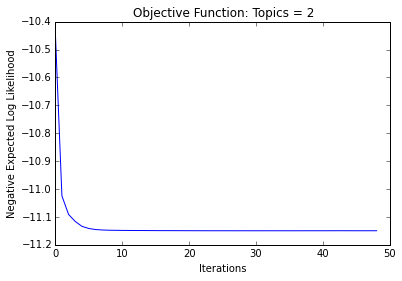
\includegraphics[width=0.6\textwidth]{output_10_2.png}
	\caption{Objective function minimization: $K = 2$ topics, 50 iterations}
\end{figure}

\noindent
topic 0 ['29138 universityoftennessee', '24417 sciences', '26455 studi', '21615 projected', '23314 researched'] \\
topic 1 ['6270 database', '26458 studio', '21615 projected', '26460 studying', '23314 researched'] \\

\newpage

\begin{figure}
	\centering
	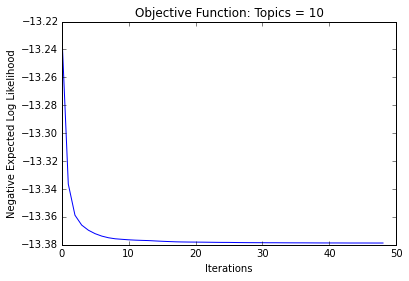
\includegraphics[width=0.6\textwidth]{output_6_2.png}
	\caption{Objective function minimization: $K = 10$ topics, 50 iterations}
\end{figure}

\noindent
topic 0 [genealogical, proteomics', '3725 cellular', '21749 proteins', '3722 celle'] \\
topic 1 ['25801 specifiable', '6270 database', '26460 studying', '21615 projected', '23314 researched'] \\
topic 2 ['29138 universityoftennessee', '21583 programing', '21615 projected', '3984 chemists', researched] \\
topic 3 ['20416 phased', '21615 projected', '16448 materiel', '12380 higham', '23314 researched'] \\
topic 4 ['21583 programing', '23314 researched', '21615 projected', '24417 sciences', '26455 studi'] \\
topic 5 ['16905 metis', '21615 projected', '21502 problemsolving', '27260 systemwide', '23314 researched'] \\
topic 6 ['21615 projected', '11389 geons', '26460 studying', '23314 researched', '27749 thep'] \\
topic 7 ['27749 thep', '21691 property', '27260 systemwide', '26460 studying', '23314 researched'] \\
topic 8 ['21785 provided', '21615 projected', '26460 studying', '6270 database', '23314 researched'] \\
topic 9 ['21583 programing', '26978 supportable', '26455 studi', '29138 universityoftennessee', '23314 researched'] \\

\newpage

\begin{figure}
	\centering
	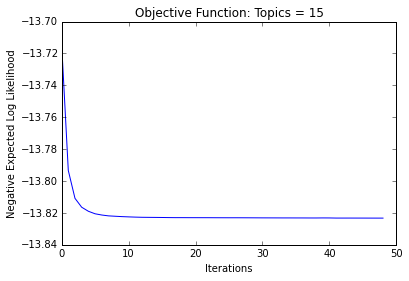
\includegraphics[width=0.6\textwidth]{output_7_2.png}
	\caption{Objective function minimization: $K = 15$ topics, 50 iterations}
\end{figure}

\noindent
topic 0 ['11294 genealogical', '21750 proteomics', '3725 cellular', '3722 celle', '21749 proteins'] \\
topic 1 ['13527 informational', '26460 studying', '6270 database', '21615 projected', '23314 researched'] \\
topic 2 ['17327 modelbased', '21615 projected', '26460 studying', '23314 researched', '6270 database'] \\
topic 3 ['27248 systematic', '11294 genealogical', '21749 proteins', '3722 celle', '3725 cellular'] \\
topic 4 ['21785 provided', '26460 studying', '21615 projected', '6270 database', '23314 researched'] \\
topic 5 ['21583 programing', '21615 projected', '23314 researched', '26455 studi', '24417 sciences'] \\
topic 6 ['26460 studying', '21502 problemsolving', '21615 projected', '27260 systemwide', '23314 researched'] \\
topic 7 ['21615 projected', '26460 studying', '21502 problemsolving', '23314 researched', '27749 thep'] \\
topic 8 ['2571 biomass', '21583 programing', '29138 universityoftennessee', '26455 studi', '23314 researched'] \\
topic 9 ['30075 watercolor', '26460 studying', '18998 oceanic', '23314 researched', '3464 carbonell'] \\
topic 10 ['20670 planted', '11340 genetically', '26460 studying', '23314 researched', '25801 specifiable'] \\
topic 11 ['21615 projected', '29138 universityoftennessee', '15083 laborious', '26455 studi', '23314 researched'] \\
topic 12 ['6270 database', '27248 systematic', '6924 designate', '27260 systemwide', '23314 researched'] \\
topic 13 ['27248 systematic', '6924 designate', '21615 projected', '12380 higham', '23314 researched'] \\
topic 14 ['26460 studying', '21691 property', '16448 materiel', '3984 chemists', '23314 researched'] \\

\newpage

\begin{figure}
	\centering
	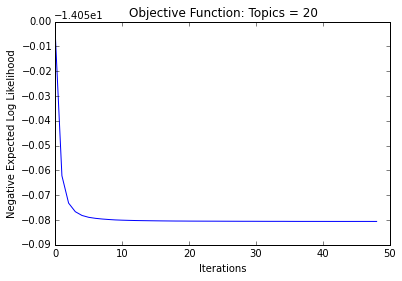
\includegraphics[width=0.6\textwidth]{output_8_2.png}
	\caption{Objective function minimization: $K = 20$ topics, 50 iterations}
\end{figure}

\noindent
topic 0 ['26460 studying', '27260 systemwide', '21691 property', '16143 magnetically', '23314 researched'] \\
topic 1 ['21615 projected', '3984 chemists', '26455 studi', '29138 universityoftennessee', '23314 researched'] \\
topic 2 ['21785 provided', '21615 projected', '26460 studying', '23314 researched', '6270 database'] \\
topic 3 ['21615 projected', '21691 property', '16448 materiel', '3984 chemists', '23314 researched'] \\
topic 4 ['29138 universityoftennessee', '21583 programing', '5099 conferences', '26455 studi', '23314 researched'] \\
topic 5 ['16905 metis', '747 algorithmus', '27260 systemwide', '21502 problemsolving', '23314 researched'] \\
topic 6 ['27248 systematic', '21615 projected', '6924 designate', '6270 database', '23314 researched'] \\
topic 7 ['11389 geons', '21502 problemsolving', '26460 studying', '23314 researched', '27749 thep'] \\
topic 8 ['6270 database', '26460 studying', '26978 supportable', '21615 projected', '23314 researched'] \\
topic 9 ['26978 supportable', '4607 colleges', '29138 universityoftennessee', '18264 networkbased', '23314 researched'] \\
topic 10 ['15083 laborious', '21615 projected', '4974 computeraided', '26455 studi', '23314 researched'] \\
topic 11 ['21750 proteomics', '23314 researched', '21749 proteins', '3722 celle', '3725 cellular'] \\
topic 12 ['21615 projected', '18998 oceanic', '26460 studying', '6270 database', '23314 researched'] \\
topic 13 ['27248 systematic', '27260 systemwide', '6270 database', '21615 projected', '23314 researched'] \\
topic 14 ['21750 proteomics', '7714 dnf', '11337 genesis', '21749 proteins', '11294 genealogical'] \\
topic 15 ['16448 materiel', '21615 projected', '19298 optically', '12380 higham', '23314 researched'] \\
topic 16 ['13527 informational', '17350 modeltheoretic', '6270 database', '21615 projected', '23314 researched'] \\
topic 17 ['20945 por', '26460 studying', '20670 planted', '23314 researched', '25801 specifiable'] \\
topic 18 ['16457 mathematik', '27466 teaches', '21615 projected', '26455 studi', '24417 sciences'] \\
topic 19 ['6270 database', '17327 modelbased', '21615 projected', '26460 studying', '23314 researched'] \\

\newpage

\begin{figure}
	\centering
	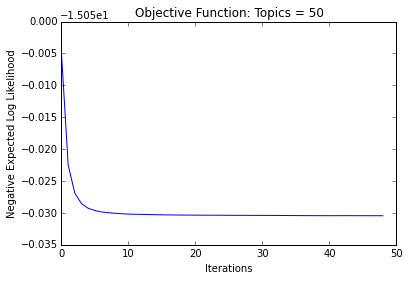
\includegraphics[width=0.6\textwidth]{output_9_2.png}
	\caption{Objective function minimization: $K = 50$ topics, 50 iterations}
\end{figure}


\clearpage
\begin{problem}[Calibration, 1pt]
Approximately how long did this homework take you to complete?
\end{problem}

20 hours

\end{document}